\begin{figure}[t!]
    \centering
        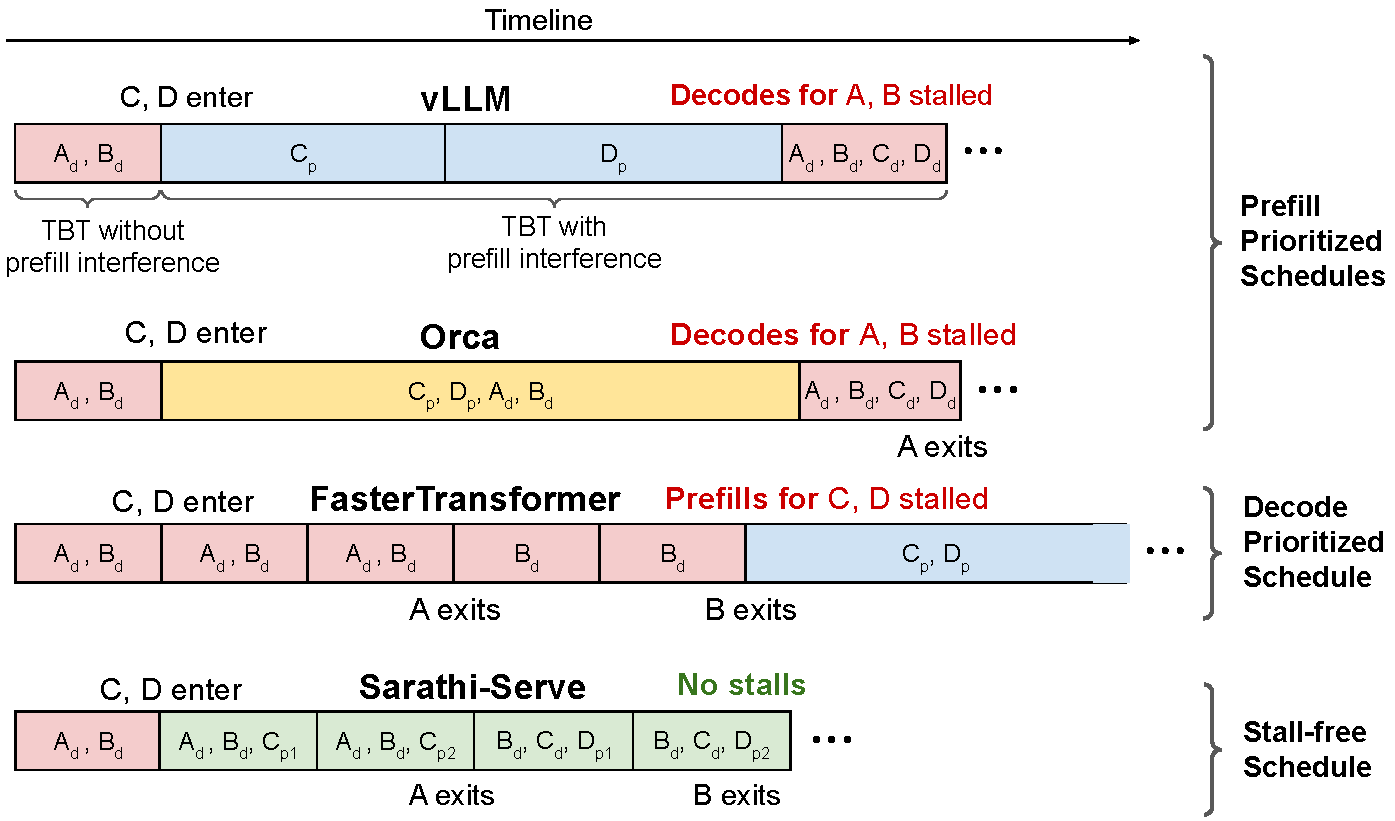
\includegraphics[width=0.47\textwidth]{figures/sarathi_server_timeline.pdf}
    \caption{A generation stall occurs when one or more prefills are scheduled in between consecutive decode iterations of a request. A, B, C and D represent different requests. Subscript $d$ represents a decode iteration, $p$ represents a full prefill and $p0$, $p1$ represent two chunked prefills of a given prompt. vLLM induces generation stalls by scheduling as many prefills as possible before resuming ongoing decodes. Despite supporting hybrid batches, Orca cannot mitigate generation stalls because the execution time of batches containing long prompts remains high. FasterTransformer is free of generation stalls as it finishes all ongoing decodes before scheduling a new prefill but compromises on throughput due to low decode batch size. In contrast, \sysname generates a schedule that eliminates generation stalls yet delivers high throughput.}
        \label{fig:motivation:generationstalls}
\end{figure}
